\chapter{被恩典帶入榮耀（21:1-22:21）}

我們終於來到新天新地\idx{13}{新天新地}了。有人可能會問：「我連今生都還沒有走完，為什麼現在就要盼望永生裡的新天新地呢？」

讓我打一個簡單的比方。假設你準備搬進一個寬敞、美麗的新家。新家已經預備好了，你也知道將來要住在那裡。可是家中的孩子和青少年，卻捨不得離開現在熟悉的房子。他們可能會說：「我住在這裡不是很好嗎？為什麼一定要搬走？」你會不會因此告訴他：「既然如此，就不要搬家了。」當然不會。你反而會帶他去看看新家，讓他知道將來要住的是怎樣的地方；你甚至會和他一起期待搬家的那一天。

希伯來書11:16說我們在地上「是客旅、是寄居的。」而我們是要「羨慕一個更美的家鄉、就是在天上的，」並且「神已經給他們預備了一座城。」主耶穌要離世的時候，也告訴我們「我去是為你們預備地方。」（約翰福音14:2）我們對新天新地的盼望也是如此。

我們並不是因為厭惡今生，才盼望將來。相反地，我們是在今生經歷神的恩典\idx{10}{恩典}、認識基督、愛人、服事主。但我們知道，這一切仍不是故事的終點。
神已經為祂的子民預備了一個更美的家鄉。那是神最終更新天地、與祂的子民永遠同住的榮耀\idx{14}{榮耀}居所。
所以，基督徒可以一面珍惜今天，一面期待那一天；一面忠心走完今生的道路，一面抬頭仰望將來的榮耀。


\begin{figure}[htbp]
    \centering
    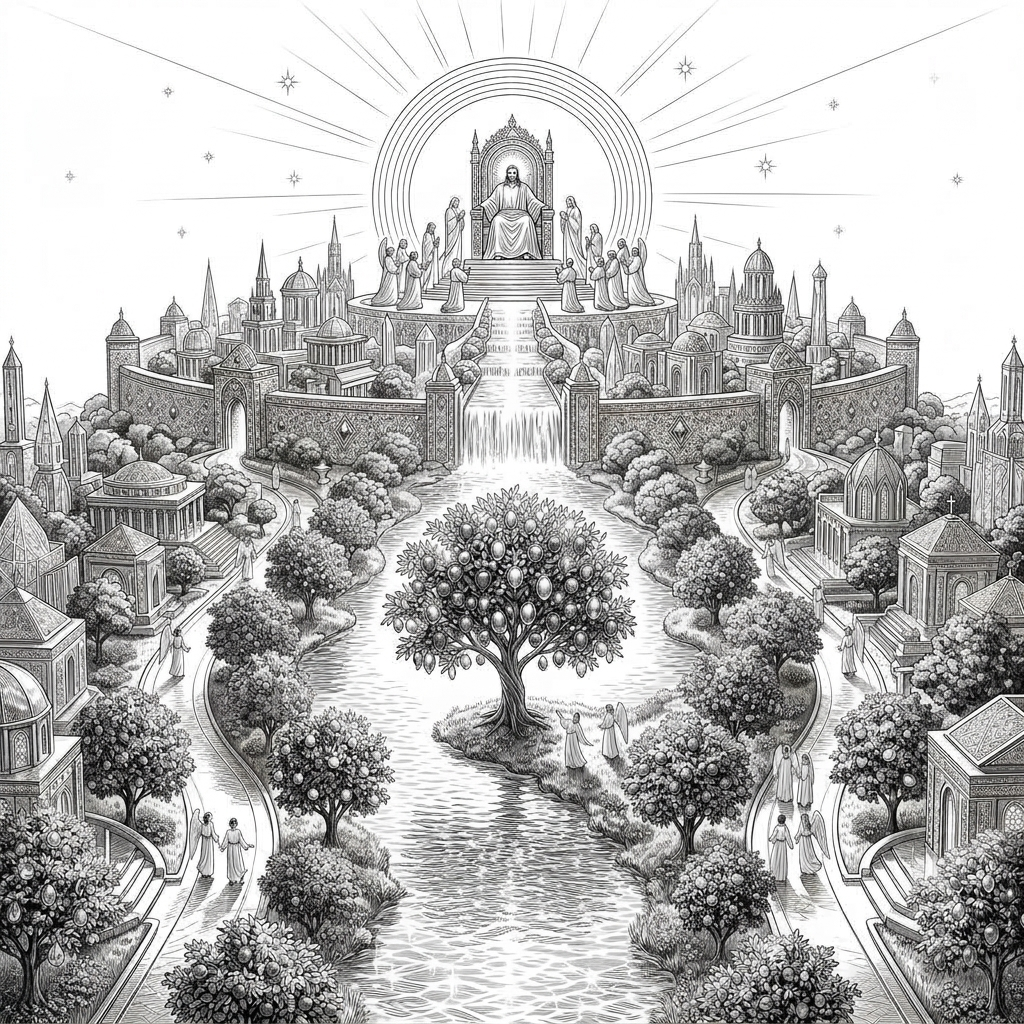
\includegraphics[
    width=1\textwidth, 
    trim=0 0 0 0, 
    clip]{images/tree_of_life.jpg}
\end{figure}



\section{一切更新，神與人同住}

\begin{ScriptureBox2}{圈出21:1–4中一切「不再有」的事物。坐寶座的說祂要將什麼更新？祂要白白賜給口渴的人什麼？}

\item[21:1]
\textit{我又看見一個新天新地．因為先前的天地已經過去了．海也不再有了。}

\item[21:2]
\textit{我又看見聖城新耶路撒冷由　神那裡從天而降、預備好了、就如新婦妝飾整齊、等候丈夫。}

\item[21:3]
\textit{我聽見有大聲音從寶座出來說、看哪、　神的帳幕在人間．他要與人同住、他們要作他的子民、　神要親自與他們同在、作他們的　神．}

\item[21:4]
\textit{神要擦去他們一切的眼淚．不再有死亡、也不再有悲哀、哭號、疼痛、因為以前的事都過去了。}

\item[21:5]
\textit{坐寶座的說、看哪、我將一切都更新了。又說、你要寫上．因這些話是可信的、是真實的。}

\item[21:6]
\textit{他又對我說、都成了。我是阿拉法、我是俄梅戛、我是初、我是終。我要將生命泉的水白白賜給那口渴的人喝。}

\item[21:7]
\textit{得勝的、必承受這些為業．我要作他的　神、他要作我的兒子。}

\item[21:8]
\textit{惟有膽怯的、不信的、可憎的、殺人的、淫亂的、行邪術的、拜偶像的、和一切說謊話的、他們的分就在燒著硫磺的火湖裡．這是第二次的死。}

\end{ScriptureBox2}

我們看到的一個重要的字，是「新天新地\idx{13}{新天新地}」、「新耶路撒冷\idx{13}{新耶路撒冷}」裡的「新」。這個「新」究竟是什麼意思？如果我們還是原來的「舊人」，帶著舊的生命、舊的性情、舊的罪進入新天新地，豈不是很不相稱嗎？所以，神不只是更新天地，也要把祂的子民生命中更新，使我們成為與祂永遠同住的人。保羅說：「所以我們不喪膽。外體雖然毀壞，內心卻一天新似一天。」（哥林多後書4:16）我們不是到了新天新地才開始更新，而是今天就已經在基督裡經歷更新；到了那一天，神要把這更新帶到完全。

我們可以想到十字架上的那個強盜。他原本是罪犯，與耶穌一同被釘十字架。然而，就在生命最後的時刻，他看見了與他同釘的耶穌，承認自己的罪，並求主記念他。耶穌對他說：「今日你要同我在樂園裡了。」（路加福音23:43）這個人沒有時間重新建立自己的人生，也沒有機會靠自己的行為證明自己已經改變；但他的心轉向了基督。他從一個犯罪的人，成為一個仰望基督、信靠基督的人。這就是恩典\idx{10}{恩典}所帶來的更新。所以，新天新地所迎接的，不是一群仍然愛慕罪惡的「舊人」，而是神已經在基督裡更新、如今仍在被祂更新，並且將來要完全得榮耀\idx{14}{榮耀}的子民。

更新一切的是誰呢？祂說「成了」。祂說「我是阿拉法、我是俄梅戛、我是初、我是終。」祂是「將生命泉的水白白賜給那口渴的人喝。」祂是在約翰福音4:14 雅各井邊，對那位婦人說「人若喝我所賜的水就永遠不渴．我所賜的水、要在他裡頭成為泉源、直湧到永生。」

\section{新婦就是新耶路撒冷}

\begin{ScriptureBox2}{數一數21:12–21中所有的「十二」。門上寫著誰的名字？根基上又寫著誰的名字？}

\item[21:9]
\textit{拿著七個金碗、盛滿末後七災的七位天使中、有一位來對我說、你到這裡來、我要將新婦、就是羔羊的妻、指給你看。}

\item[21:10]
\textit{我被聖靈感動、天使就帶我到一座高大的山將那由　神那裡從天而降的聖城耶路撒冷指示我。}

\item[21:11]
\textit{城中有　神的榮耀．城的光輝如同極貴的寶石、好像碧玉、明如水晶．}

\item[21:12]
\textit{有高大的牆．有十二個門、門上有十二位天使．門上又寫著以色列十二個支派的名字．}

\item[21:13]
\textit{東邊有三門．北邊有三門．南邊有三門．西邊有三門。}

\item[21:14]
\textit{城牆有十二根基、根基上有羔羊十二使徒的名字。}

\item[21:15]
\textit{對我說話的拿著金葦子當尺、要量那城、和城門城牆。}

\item[21:16]
\textit{城是四方的、長寬一樣、天使用葦子量那城、共有四千里．長寬高都是一樣。}

\item[21:17]
\textit{又量了城牆、按著人的尺寸、就是天使的尺寸、共有一百四十四肘。}

\item[21:18]
\textit{牆是碧玉造的．城是精金的、如同明淨的玻璃。}

\item[21:19]
\textit{城牆的根基是用各樣寶石修飾的。第一根基是碧玉．第二是藍寶石．第三是綠瑪瑙．第四是綠寶石．}

\item[21:20]
\textit{第五是紅瑪瑙．第六是紅寶石．第七是黃璧璽．第八是水蒼玉．第九是紅璧璽．第十是翡翠．第十一是紫瑪瑙．第十二是紫晶。}

\item[21:21]
\textit{十二個門是十二顆珍珠．每門是一顆珍珠．城內的街道是精金、好像明透的玻璃。}

\end{ScriptureBox2}


聖城\idx{13}{聖城}由天而降，充滿光輝，大有榮耀\idx{14}{榮耀}。約翰仔細觀看。每一面有三個門，寫了以色列\idx{05}{以色列}十二個支派的名字．約翰看的非常仔細。城牆有十二根基、根基上有羔羊\idx{10}{羔羊}十二使徒的名字。這不禁使我們想起，耶穌對彼得說：「你是彼得，我要把我的教會建造在這磐石上；陰間\idx{11}{陰間}的權柄不能勝過他。」（馬太福音16:18）。聖城新耶路撒冷\idx{13}{新耶路撒冷}不僅有十二根基（代表新約的十二使徒），還有十二個門（上面寫著以色列十二個支派的名字）。這表明上帝救贖\idx{11}{救贖}計畫是完整的，將舊約的以色列選民與新約的基督教會，完美地結合在同一個榮耀的居所中。這段經文提醒著所有基督徒，教會的信仰是有根有基的，正是建立在使徒和先知的根基上，並且以耶穌基督自己為房角石（以弗所書 2:20）。

\begin{InDepth}
\InDepthHeading{新耶路撒冷有多大？}

這裡特別給了城的尺寸，那是象徵完全、聖潔、無缺。這城是一個正立方體，長、寬、高都相等約有「四千里」。
以現代的尺寸來換算，約1,400 英里。\footnotemark

\begin{center}
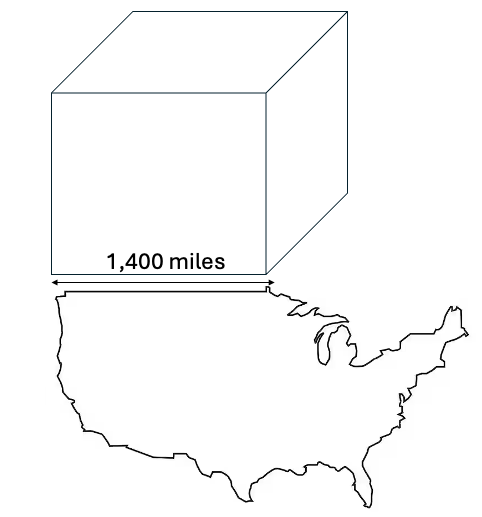
\includegraphics[width=0.6\linewidth]{images/new_jesusalem_US.png}
\end{center}

美國東西方向寬度的一半約1,400 英里。現在，
請想像這樣一座巨大的立方體。長、寬、高是1,400 英里。
那個燦爛浩大的城。
\end{InDepth}
% Footnote text for the mark in the box above
\footnotetext{希臘文原文是一萬二千 stadia。和合本中文聖經翻譯者採用了一個換算：3 stadia ≈ 1 里。12,000 stadia ÷ 3 = 4,000 里。所以才有「共有四千里」。}

並且，
啟示錄7:9告訴我們那站在寶座\idx{20}{寶座}和羔羊面前的，是「沒有人能數過來的各國、各族、各民、各方」的群眾。
是所有在永生中的人可以自由行走的。

這個簡單的比較，只是幫助我們稍微想像聖城的宏偉與廣大。當我們思想這樣的尺度時，可以驚嘆神的創造何等浩大、祂為祂子民所預備的榮耀何等超越我們的想像。
正如保羅所說：「神為愛他的人所預備的是眼睛未曾看見，耳朵未曾聽見，人心也未曾想到的。」（哥林多前書2:9）




\section{神自己就是城的殿}

\begin{ScriptureBox2}{約翰在城內沒有看見什麼？為什麼？城的光從哪裡來？誰才得進那城？}

\item[21:22]
\textit{我未見城內有殿、因主　神全能者、和羔羊、為城的殿。}

\item[21:23]
\textit{那城內又不用日月光照．因有　神的榮耀光照．又有羔羊為城的燈。}

\item[21:24]
\textit{列國要在城的光裡行走．地上的君王必將自己的榮耀歸與那城。}

\item[21:25]
\textit{城門白晝總不關閉．在那裡原沒有黑夜。}

\item[21:26]
\textit{人必將列國的榮耀尊貴歸與那城。}

\item[21:27]
\textit{凡不潔淨的、並那行可憎與虛謊之事的、總不得進那城．只有名字寫在羔羊生命冊上的纔得進去。}

\end{ScriptureBox2}

在城中的人，是蒙恩得救的人；他們的名字已經寫在羔羊\idx{10}{羔羊}生命冊\idx{05}{生命冊}上。 他們是神恩典\idx{10}{恩典}的工作。祂在基督裡揀選、呼召、赦免並保守祂的子民，最終把他們帶進這座永恆的城。因此，新天新地\idx{13}{新天新地}中的人既有共同的身分，都是羔羊所救贖\idx{11}{救贖}的子民；又保留各族的豐富與多樣。差異不再成為分裂的原因，反而成為共同榮耀\idx{14}{榮耀}神的豐富色彩。這是一個何等美麗的畫面！

\begin{ReaderQuestion}
從伊甸園、會幕、聖殿、基督道成肉身，一直到新天新地，你看見神與人同住的應許如何逐步展開？
\end{ReaderQuestion}

\section{生命的河與生命樹}

\begin{ScriptureBox2}{生命水的河從哪裡流出來？劃出22:3–5中神的僕人要做的事和要看見的。}

\item[22:1]
\textit{天使又指示我在城內街道當中一道生命水的河、明亮如水晶、從　神和羔羊的寶座流出來。}

\item[22:2]
\textit{在河這邊與那邊有生命樹、結十二樣果子、〔樣或作回〕每月都結果子．樹上的葉子乃為醫治萬民。}

\item[22:3]
\textit{以後再沒有咒詛．在城裡有　神和羔羊的寶座．他的僕人都要事奉他．}

\item[22:4]
\textit{也要見他的面．他的名字必寫在他們的額上。}

\item[22:5]
\textit{不再有黑夜．他們也不用燈光日光．因為主　神要光照他們．他們要作王、直到永永遠遠。}

\end{ScriptureBox2}

22:1–2首先把讀者帶回《創世記》的伊甸園\idx{06}{伊甸園}。在伊甸園中有生命樹\idx{05}{生命樹}，也有河流。生命水\idx{05}{生命水}的河是「從神和羔羊\idx{10}{羔羊}的寶座\idx{20}{寶座}流出來。」人的生命倚靠神並享受神的福樂，是受造的恩典\idx{10}{恩典}。這裡的生命樹「每月都結果子」，持續供應人的生命，使人永遠豐盛。

「樹上的葉子乃為醫治萬民」並不是說新創造中還存在疾病。這個果子吃了使人愉悅，比較像是超級維他命的概念。吃了的人精神百倍，心裡暢快。\footnote{MacArthur, J. (2007).}

\begin{InDepth}
\InDepthHeading{失樂園與復樂園}

22:3說：「以後再沒有咒詛」，使我們想到創世記3章，罪進入世界，咒詛隨之而來；啟示錄22章，救贖\idx{11}{救贖}完成，咒詛被徹底除去。如果我們比較兩者，我們可以得到非常好的理解：

\par\medskip\noindent
\begin{minipage}{\linewidth}
\centering\small
\renewcommand{\arraystretch}{1}\setlength{\tabcolsep}{4pt}
\captionof{table}{創世記3章與啟示錄21--22章}
\label{tab:genesis3-rev21-22-zh}
\begin{tabularx}{\linewidth}{>{\raggedright\arraybackslash}X
                              >{\raggedright\arraybackslash}X}
\hline
創世記3章 & 啟示錄21--22章 \\
\hline
罪進入世界 & 一切都更新 \\
咒詛臨到 & 不再有咒詛 \\
被趕出伊甸園 & 進入聖城\idx{13}{聖城} \\
不能吃生命樹 & 得著生命樹 \\
與神隔絕 & 神與人同住 \\
死亡進入世界 & 不再有死亡 \\
蛇引誘人 & 撒但\idx{15}{撒但}完全敗亡 \\
人失去神的面 & 「也要見他的面」 \\
\hline
\end{tabularx}
\end{minipage}
\end{InDepth}


\section{這書不可封閉}

\begin{ScriptureBox2}{在這段經文中，耶穌說了幾次「我必快來」？圈出每一個「有福了」，並留意誰是有福的。}

\item[22:6]
\textit{天使又對我說、這些話是真實可信的．主就是眾先知被感之靈的　神、差遣他的使者、將那必要快成的事指示他僕人。}

\item[22:7]
\textit{看哪、我必快來。凡遵守這書上預言的有福了。}

\item[22:8]
\textit{這些事是我約翰所聽見所看見的．我既聽見看見了、就在指示我的天使腳前俯伏要拜他。}

\item[22:9]
\textit{他對我說、千萬不可．我與你、和你的弟兄眾先知、並那些守這書上言語的人、同是作僕人的．你要敬拜　神。}

\item[22:10]
\textit{他又對我說、不可封了這書上的預言．因為日期近了。}

\item[22:11]
\textit{不義的、叫他仍舊不義．污穢的、叫他仍舊污穢．為義的、叫他仍舊為義．聖潔的、叫他仍舊聖潔。}

\item[22:12]
\textit{看哪、我必快來．賞罰在我、要照各人所行的報應他。}

\item[22:13]
\textit{我是阿拉法、我是俄梅戛、我是首先的、我是末後的、我是初、我是終。}

\item[22:14]
\textit{那些洗淨自己衣服的有福了、可得權柄能到生命樹那裡、也能從門進城。}

\item[22:15]
\textit{城外有那些犬類、行邪術的、淫亂的、殺人的、拜偶像的、並一切喜好說謊言編造虛謊的。}

\end{ScriptureBox2}

現在，啟示錄是直接對你我勸勉。天使宣告：「這些話是真實可信的。」因為這卷書是要讓神的百姓公開宣讀、聽見遵守而得福的。

這裡，我們又一次聽見耶穌宣告祂自己的身分：「我是阿拉法，我是俄梅戛，我是首先的，我是末後的，我是初，我是終。」阿拉法（Alpha）是希臘文的第一個字母，俄梅戛（Omega）是最後一個字母。整個世界的歷史都在祂的掌權之下。從創世直到新天新地\idx{13}{新天新地}，從十字架到榮耀\idx{14}{榮耀}，沒有任何事情超出祂的計畫。

「不義的，叫他仍舊不義……聖潔的，叫他仍舊聖潔。」這句話的意思是說，義人與惡人個別的心思意念完全顯露付諸行動。人的生命所結出的果子，最終顯明他是否屬於羔羊\idx{10}{羔羊}。人在今生所持守的道路，將在永恆中顯明其最終的歸屬。

\section{最後的福音邀請：口渴的人都可以來}

\begin{ScriptureBox2}{耶穌在22:16如何描述自己？誰說「來」？誰被邀請取生命的水喝？}

\item[22:16]
\textit{我耶穌差遣我的使者為眾教會將這些事向你們證明。我是大衛的根、又是他的後裔．我是明亮的晨星。}

\item[22:17]
\textit{聖靈和新婦都說來。聽見的人也該說來。口渴的人也當來．願意的都可以白白取生命的水喝。}

\end{ScriptureBox2}


最後，啟示錄再提出邀請，是向每一個讀到這卷書、仍然「口渴」的人發出最美好的福音呼召：「口渴的人也當來；願意的，都可以白白取生命的水喝。」（啟 22:17）這讓我們想起主耶穌在井旁對撒瑪利亞婦人所說的話：「人若喝我所賜的水就永遠不渴。我所賜的水，要在他裡頭成為泉源，直湧到永生。」（約 4:14）神希望將人帶到祂永生的榮耀\idx{14}{榮耀}裡，飲用祂賜給人的生命水\idx{05}{生命水}，直到永生。

\begin{ReaderQuestion}
如果你要向一位尚未信主、但正在人生中感到「口渴」的人解釋這句話，你會怎樣說？這節經文如何顯明福音是恩典，而不是靠人的功德換取？
\end{ReaderQuestion}

\section{「主耶穌啊，我願你來」}

\begin{ScriptureBox2}{關於這書上的預言，有什麼警告？教會在22:20如何回應耶穌的應許？}

\item[22:18]
\textit{我向一切聽見這書上預言的作見證、若有人在這預言上加添甚麼、　神必將寫在這書上的災禍加在他身上．}

\item[22:19]
\textit{這書上的預言、若有人刪去甚麼、　神必從這書上所寫的生命樹、和聖城、刪去他的分。}

\item[22:20]
\textit{證明這事的說、是了．我必快來。阿們。主耶穌阿、我願你來。}

\item[22:21]
\textit{願主耶穌的恩惠、常與眾聖徒同在。阿們。}

\end{ScriptureBox2}


書的結語是主耶穌的「我必快來」，以及人的回應「我願你來」。使我們想起《雅歌》中良人與女子彼此渴望的對話。新婦\idx{13}{新婦}所盼望的，不只是婚宴本身，而是良人親自來到。同樣，教會所等候的，是那位愛我們、為我們捨己、又從死裡復活的羔羊\idx{10}{羔羊}親自來到。我們何其有幸，可以與主對話，祂的「我必快來」，是我的持守，是我在患難中的力量。

\begin{ReaderQuestion}
對你而言，「主耶穌啊，我願你來」不只是對未來的盼望，也可以如何成為今天生活的禱告？在工作、家庭、苦難、服事和面對不確定的未來時，這個盼望可以怎樣改變我們？
\end{ReaderQuestion}
